\documentclass[aspectratio=169, table]{beamer}

\usepackage{colortbl}
\usepackage{xcolor}
\usepackage{listings}
\usepackage{tikz}
\usepackage{pgfplots}
\usepgfplotslibrary{polar}
\usetikzlibrary{arrows.meta, positioning, calc}

\usetheme{Pradita}



\lstdefinelanguage{bash} {
	keywords={},
	basicstyle=\ttfamily\small,
	keywordstyle=\color{blue}\bfseries,
	ndkeywords={iex},
	ndkeywordstyle=\color{purple}\bfseries,
	sensitive=true,
	commentstyle=\color{gray},
	stringstyle=\color{red},
	numbers=left,
	numberstyle=\tiny\color{gray},
	breaklines=true,
	frame=lines,
	backgroundcolor=\color{lightgray!10},
	tabsize=2,
	comment=[l]{\#},
	morecomment=[s]{/*}{*/},
	commentstyle=\color{gray}\ttfamily,
	stringstyle=\color{purple}\ttfamily,
	showstringspaces=false
}

% Define Python language style for listings
\lstdefinestyle{PythonStyle}{
    language=Python,
    basicstyle=\ttfamily\footnotesize,
    keywordstyle=\color{blue}\bfseries,
    commentstyle=\color{gray}\itshape,
    stringstyle=\color{red},
    showstringspaces=false,
    breaklines=true,
    frame=lines,
    numbers=left,
    numberstyle=\tiny\color{gray},
    backgroundcolor=\color{lightgray!10},
    tabsize=4,
    captionpos=b
}


\title{\Huge Observability \\
	\vspace{10pt}}
\subtitle{IT30213 - Advanced Software Engineering \& DevOps}
%\date[Serial]{Penggunaan Large Language Model untuk Pengajaran}
\author{\textbf{Alfa Yohannis}}
\begin{document}
	
	\frame{\titlepage}
	

	\begin{frame}[fragile]
		\frametitle{Contents}
		\vspace{20pt}
		\begin{columns}[t]
			\column{0.5\textwidth}
			\tableofcontents[sections={1-5}]
			
			\column{0.5\textwidth}
			\tableofcontents[sections={6-20}]
		\end{columns}
	\end{frame}
	
	\begin{frame}{\hfill}
		\centering
		\Huge{\textbf{How to know that\\our systems work properly?}}
	\end{frame}
	
	\section{Introduction}
	
	\begin{frame}{\hfill}
		\centering
		\Huge{\textbf{Introduction}}
	\end{frame}
	
	\begin{frame}{Konsep Dasar Observabilitas}
	\vspace{6pt}
	\begin{itemize}
		\item \textbf{Monitoring} berfokus pada kondisi yang sudah diketahui, menggunakan metrik dan ambang batas untuk menjawab apakah sistem normal atau tidak.
		\item \textbf{Observabilitas} berfokus pada penalaran kondisi internal sistem dari sinyal runtime, termasuk situasi yang tidak diprediksi sebelumnya.
		\item Monitoring melihat komponen secara terpisah; observabilitas mengaitkan perilaku lintas komponen.
		\item \textbf{Metrik} menunjukkan tren agregat, \textbf{log} memberi konteks peristiwa, dan \textbf{trace} menelusuri alur eksekusi end-to-end.
		\item Observabilitas bersifat \textbf{bottom-up}: memahami sistem dari eksekusi nyata, bukan dari asumsi desain.
	\end{itemize}
	
	\vspace{4pt}
	{\footnotesize Monitoring menjawab \emph{apa yang salah}, observabilitas menjawab \emph{mengapa itu terjadi}}
\end{frame}

	\section{Arsitektur Sistem Studi Kasus}
	
	\begin{frame}{\hfill}
		\centering
		\Huge{\textbf{Arsitektur Sistem Studi Kasus}}
	\end{frame}


\begin{frame}{Arsitektur Sistem Studi Kasus}
	\vspace{20pt}
	\centering
	\scalebox{0.9}{
	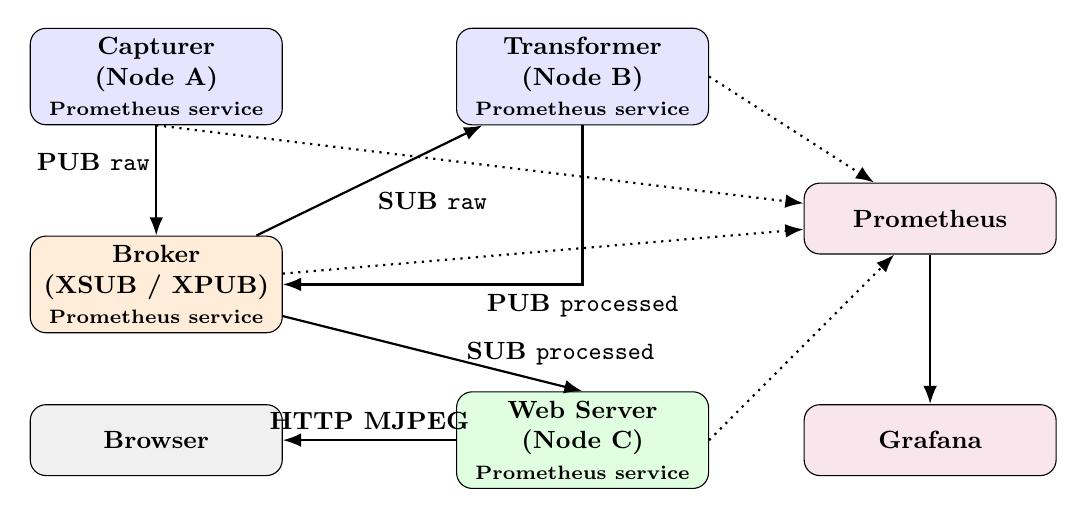
\begin{tikzpicture}[
	  font=\small\bfseries,
	  node distance=9mm and 12mm,
	  box/.style={
	    draw,
	    rounded corners=2mm,
	    align=center,
	    minimum width=32mm,
	    minimum height=9mm,
	    fill=blue!10
	  },
	  brokerbox/.style={box,fill=orange!15},
	  webbox/.style={box,fill=green!12},
	  browserbox/.style={box,fill=gray!12},
	  extbox/.style={box,fill=purple!10},
	  arrow/.style={-Latex,thick},
	  dottedarrow/.style={-Latex,thick,dotted}
	]
	
	\node[box ] (transformer) {Transformer\\(Node B)\\{\scriptsize Prometheus service}};
	\node[box,left=of transformer, xshift=-10mm] (capturer) {Capturer\\(Node A)\\{\scriptsize Prometheus service}};
	\node[brokerbox, below=of capturer, yshift=-5mm] (broker) {Broker\\(XSUB / XPUB)\\{\scriptsize Prometheus service}};
	
	\node[browserbox,below=of broker] (browser) {Browser};
	\node[webbox,right=of browser, xshift=10mm](web) {Web Server\\(Node C)\\{\scriptsize Prometheus service}};
	
	\node[extbox,right=of web] (grafana) {Grafana};
	\node[extbox,above=of grafana, yshift=10mm] (prom) {Prometheus};
	
	\draw[arrow] (capturer) -- node[above, xshift=-8mm]{PUB \texttt{raw}} (broker);
	\draw[arrow] (broker) -- node[above, yshift=-5mm, xshift=8mm]{SUB \texttt{raw}} (transformer);
	\draw[arrow] (transformer.south) |- node[below]{PUB \texttt{processed}} (broker.east);
	\draw[arrow] (broker) -- node[right,xshift=3mm]{SUB \texttt{processed}} (web.north);
	\draw[arrow] (web.west) -- node[above]{HTTP MJPEG} (browser.east);
	
	\draw[dottedarrow] (capturer.south) -- (prom);
	\draw[dottedarrow] (broker) -- (prom);
	\draw[dottedarrow] (transformer.east) -- (prom);
	\draw[dottedarrow] (web.east) -- (prom);
	\draw[arrow] (prom) -- (grafana);
	
	\end{tikzpicture}
	}
	
	\vspace{3pt}
	{\footnotesize Arsitektur publish--subscribe dengan observabilitas tertanam dan komponen eksternal}
\end{frame}

\begin{frame}{Prometheus dan Grafana}
	\vspace{20pt}
	\begin{itemize}
		\item \textbf{Prometheus} digunakan sebagai komponen observabilitas terpusat yang mengumpulkan metrik runtime dari setiap node (Capturer, Broker, Transformer, Web Server) dengan model \emph{pull-based}.
		\item Metrik disimpan sebagai \emph{time-series data}, sehingga memungkinkan analisis tren, lonjakan beban, latensi, dan indikasi kegagalan parsial tanpa ikut dalam alur data aplikasi.
		\item \textbf{Grafana} berperan sebagai lapisan visualisasi yang melakukan kueri ke Prometheus dan menyajikan perilaku sistem melalui dashboard yang mudah diinterpretasikan.
	\end{itemize}
	
	\vspace{4pt}
	{\footnotesize Observabilitas diposisikan sebagai praktik bottom-up berbasis sinyal runtime}
\end{frame}

	\section{Tahapan Eksperimen}
	
	\begin{frame}{\hfill}
		\centering
		\Huge{\textbf{Tahapan Eksperimen}}
	\end{frame}

\begin{frame}{Langkah Implementasi Observabilitas}
	\vspace{20pt}
	\begin{enumerate}
		\item Pasang \texttt{prometheus-client} dan siapkan endpoint \texttt{/metrics} pada setiap node aplikasi.
		\item Definisikan \textbf{shared library metrik} (Counter, Gauge, Histogram) agar konsisten lintas node.
		\item Inisialisasi server metrik pada setiap node dengan port berbeda saat startup.
		\item Instrumentasikan kode runtime (capturer, broker, transformer, web) untuk mencatat throughput dan latensi.
		\item Tambahkan layanan \textbf{Prometheus} dan \textbf{Grafana} ke \texttt{docker-compose.yml}.
		\item Konfigurasikan \texttt{prometheus.yml}: target scraping berbasis nama service Docker.
		\item Hubungkan Grafana ke Prometheus sebagai data source.
		\item Amati perilaku sistem melalui endpoint aplikasi, metrik, dan dashboard Grafana.
	\end{enumerate}
\end{frame}


\begin{frame}[fragile]{Setup Prometheus}
	\vspace{20pt}
	\begin{lstlisting}[language=bash, basicstyle=\ttfamily\scriptsize]
pip install prometheus-client
	\end{lstlisting}
	
	\vspace{6pt}
	\begin{itemize}
		\item Prometheus dijalankan sebagai container terpisah.
		\item Setiap node aplikasi mengekspor endpoint \texttt{/metrics}.
		\item Prometheus melakukan scraping metrik secara periodik.
		\item Observabilitas dipisahkan dari alur data utama aplikasi.
	\end{itemize}
\end{frame}

\begin{frame}[fragile]{Shared Library Metrik}
	\vspace{20pt}
	\begin{columns}[t]
		\column{0.5\textwidth}
		\begin{lstlisting}[style=PythonStyle,basicstyle=\ttfamily\scriptsize]
# shared/metrics2.py
from prometheus_client import Counter, Gauge, Histogram

frames_in_total = Counter(
    "frames_in_total",
    "Total frames received",
    ["service"]
)

frames_out_total = Counter(
    "frames_out_total",
    "Total frames produced",
    ["service"]
)
		\end{lstlisting}
		
		\column{0.5\textwidth}
		\begin{lstlisting}[style=PythonStyle,basicstyle=\ttfamily\scriptsize, firstnumber=15]
queue_size = Gauge(
    "queue_size",
    "Approximate queue size",
    ["service", "queue"]
)

processing_seconds = Histogram(
    "processing_seconds",
    "Processing latency (seconds)",
    ["service", "stage"]
)
		\end{lstlisting}
	\vspace{6pt}
	{\footnotesize Definisi metrik dibagi per tipe namun tetap dalam satu shared library}
	\end{columns}
	

\end{frame}


\begin{frame}[fragile]{Inisialisasi Server Metrik}
	\vspace{20pt}
	\begin{lstlisting}[style=PythonStyle, basicstyle=\ttfamily\scriptsize]
from prometheus_client import start_http_server
from shared.metrics2 import frames_in_total

SERVICE = "capturer"

def init_metrics_server(port: int):
    start_http_server(port)

init_metrics_server(9101)
	\end{lstlisting}
	
	\vspace{6pt}
	\begin{itemize}
		\item Setiap node menjalankan endpoint metrik pada port berbeda.
		\item Endpoint \texttt{/metrics} diaktifkan saat startup node.
		\item Pola inisialisasi sama untuk Capturer, Broker, Transformer, dan Web.
	\end{itemize}
\end{frame}

\begin{frame}[fragile]{Penggunaan Metrik Runtime}
	\vspace{20pt}
	\begin{lstlisting}[style=PythonStyle, basicstyle=\ttfamily\scriptsize]
frames_in_total.labels(service=SERVICE).inc()

with processing_seconds.labels(
        service=SERVICE,
        stage="decode"
    ).time():
    process_frame()
	\end{lstlisting}
	
	\vspace{6pt}
	\begin{itemize}
		\item Counter merepresentasikan volume dan throughput.
		\item Histogram menangkap latensi pemrosesan.
		\item Perubahan metrik dikorelasikan dengan perilaku runtime sistem.
	\end{itemize}
\end{frame}


\begin{frame}[fragile]{Metrik pada Capturer dan Broker}
	\vspace{20pt}
	
	\textbf{Capturer (Node A)}
	\begin{lstlisting}[style=PythonStyle,basicstyle=\ttfamily\scriptsize]
from time import time
from shared.metrics2 import (frames_out_total, processing_seconds)

t0 = time()
# capture + publish frame
frames_out_total.labels(service="capturer").inc()
processing_seconds.labels(service="capturer", stage="capture_publish").observe(time() - t0)
	\end{lstlisting}
	
	\textbf{Broker}
	\begin{lstlisting}[style=PythonStyle,basicstyle=\ttfamily\scriptsize]
from shared.metrics2 import (frames_in_total, frames_out_total)

# menerima raw / processed
frames_in_total.labels(service="broker").inc()
frames_out_total.labels(service="broker").inc()
	\end{lstlisting}
\end{frame}


\begin{frame}[fragile]{Metrik pada Transformer dan Web Server}
	\vspace{20pt}
	
	\textbf{Transformer (Node B)}
	\begin{lstlisting}[style=PythonStyle,basicstyle=\ttfamily\scriptsize]
from time import time
from shared.metrics2 import (frames_in_total, frames_out_total, processing_seconds)
# saat menerima raw
frames_in_total.labels(service="transformer").inc()

t0 = time()
# transform frame
frames_out_total.labels(service="transformer").inc()
processing_seconds.labels(service="transformer", stage="transform").observe(time() - t0)
	\end{lstlisting}
	
	\textbf{Web Server (Node C)}
	\begin{lstlisting}[style=PythonStyle,basicstyle=\ttfamily\scriptsize]
from shared.metrics2 import (frames_in_total, frames_out_total)

# menerima processed dari broker
frames_in_total.labels(service="web_server").inc()
frames_out_total.labels(service="web_server").inc()
	\end{lstlisting}
\end{frame}

\begin{frame}[fragile]{Docker Compose: Prometheus dan Grafana}
	\vspace{20pt}
	\begin{columns}[t]
		\column{0.5\textwidth}
		\begin{lstlisting}[language=bash,basicstyle=\ttfamily\scriptsize]
services:
  prometheus:
    image: prom/prometheus:latest
    container_name: prometheus
    ports:
      - "9090:9090"
    volumes:
      - ./prometheus/prometheus.yml:/etc/prometheus/prometheus.yml:ro
    command:
      - "--config.file=/etc/prometheus/prometheus.yml"
    depends_on:
      - capturer
      - broker
      - transformer
      - web
		\end{lstlisting}
		
		\column{0.5\textwidth}
		\begin{lstlisting}[language=bash,basicstyle=\ttfamily\scriptsize]
  grafana:
    image: grafana/grafana:latest
    container_name: grafana
    ports:
      - "3000:3000"
    depends_on:
      - prometheus
		\end{lstlisting}
	\vspace{6pt}
	{\footnotesize Prometheus mengumpulkan metrik runtime; Grafana menyajikan visualisasi dari data yang sama dalam jaringan Docker Compose (docker-compose.yml)}
	\end{columns}
	

\end{frame}

\begin{frame}[fragile]{Konfigurasi Prometheus: Scraping Target}
	\vspace{20pt}
	\begin{columns}[t]
		\column{0.5\textwidth}
		\begin{lstlisting}[language=bash,basicstyle=\ttfamily\scriptsize]
global:
  scrape_interval: 5s
  evaluation_interval: 5s

scrape_configs:
  - job_name: "capturer"
    static_configs:
      - targets: ["capturer:9101"]

  - job_name: "broker"
    static_configs:
      - targets: ["broker:9102"]
		\end{lstlisting}
		
		\column{0.5\textwidth}
		\begin{lstlisting}[language=bash,basicstyle=\ttfamily\scriptsize]
  - job_name: "transformer"
    static_configs:
      - targets: ["transformer:9103"]

  - job_name: "web_server"
    static_configs:
      - targets: ["web:9104"]
		\end{lstlisting}
	\vspace{6pt}
	{\footnotesize Target scraping menggunakan nama service Docker Compose, bukan \texttt{localhost}}
	\end{columns}
	

\end{frame}


\begin{frame}[fragile]{Grafana: Koneksi ke Prometheus}
	\vspace{20pt}
	\begin{lstlisting}[language=bash,basicstyle=\ttfamily\scriptsize]
Data Source Type : Prometheus
URL              : http://prometheus:9090
Access           : Server (default)
	\end{lstlisting}
	
	\vspace{6pt}
	\begin{itemize}
		\item Grafana berjalan dalam jaringan Docker Compose yang sama.
		\item Alamat Prometheus diakses via nama service.
		\item Setelah koneksi aktif, metrik dapat divisualisasikan melalui dashboard.
	\end{itemize}
	
	\vspace{4pt}
	{\footnotesize Observasi sistem dilakukan secara bottom-up melalui data runtime}
\end{frame}

\begin{frame}{Titik Observasi dan Antarmuka Sistem}
	\vspace{20pt}
	\begin{columns}[t]
		\column{0.6\textwidth}
		\textbf{Antarmuka Aplikasi}
		\begin{itemize}
			\item \url{http://localhost:8000/}  
			      Antarmuka web utama aplikasi.
			\item \url{http://localhost:8000/stream.mjpg}  
			      Aliran video MJPEG hasil pemrosesan sistem.
		\end{itemize}
		
		\vspace{6pt}
		\textbf{Endpoint Metrik Runtime}
		\begin{itemize}
			\item Capturer: \url{http://localhost:9101/metrics}
			\item Broker: \url{http://localhost:9102/metrics}
			\item Transformer: \url{http://localhost:9103/metrics}
			\item Web Server: \url{http://localhost:9104/metrics}
		\end{itemize}
		
		\column{0.4\textwidth}
		\textbf{Layanan Observabilitas}
		\begin{itemize}
			\item Prometheus: \url{http://localhost:9090}  
			      Kueri dan eksplorasi metrik.
			\item Grafana: \url{http://localhost:3000}  
			      Visualisasi metrik melalui dashboard.
		\end{itemize}
		
		\vspace{8pt}
		{\footnotesize Perubahan beban, alur data, dan pemrosesan tercermin langsung pada metrik dan visualisasi}
	\end{columns}
\end{frame}

	\section{Hasil Eksperimen}
	
	\begin{frame}{\hfill}
		\centering
		\Huge{\textbf{Hasil Eksperimen}}
	\end{frame}


\begin{frame}{Analisis Komponen Pipeline}
	\vspace{20pt}
	\centering
	\setlength{\arrayrulewidth}{0.8pt}
	\arrayrulecolor{black}
	\begin{tabular}{|l|l|c|c|c|}
	\hline
	\textbf{Komponen} & \textbf{Fungsi} & \textbf{Data} & \textbf{CPU} & \textbf{Memori} \\
	\hline
	Capturer & Akuisisi + JPEG & 8.473 frame & $\sim$54\% & $\sim$128 MB \\
	\hline
	Broker & Forward pesan & 17.030 msg & $\sim$2\% & $\sim$32 MB \\
	\hline
	Transformer & Decode--transform--encode & 8.641 frame & $\sim$21\% & 45--52 MB \\
	\hline
	Web Server & Streaming MJPEG & 8.819 frame & $\sim$0\% & $\sim$193 MB \\
	\hline
	\end{tabular}
	
	\vspace{6pt}
	\begin{itemize}
		\item Capturer dan Transformer menunjukkan beban komputasi tertinggi karena operasi encoding dan pemrosesan citra.
		\item Broker memiliki overhead minimal karena hanya melakukan forwarding pesan tanpa memproses isi data.
		\item Web Server cenderung boros memori akibat buffering stream dan manajemen koneksi klien.
	\end{itemize}
\end{frame}


\begin{frame}{Dampak Jumlah Klien MJPEG}
	\vspace{20pt}
	\centering
	\setlength{\arrayrulewidth}{0.8pt}
	\arrayrulecolor{black}
	\begin{tabular}{|l|c|c|c|}
	\hline
	\textbf{Yang Diukur} & \textbf{1 Klien} & \textbf{6 Klien} & \textbf{Perubahan} \\
	\hline
	Frame diterima & 7.070 & 7.517 & $\sim$+6\% \\
	\hline
	Total data (MB) & 697 & 741 & $\sim$+6\% \\
	\hline
	Ukuran JPEG (KB) & 98,6 & 98,6 & Tetap \\
	\hline
	Latensi rata-rata (ms) & 30,1 & 30,2 & Tetap \\
	\hline
	Latensi maksimum (ms) & $\le$100 & $\le$100 & Tetap \\
	\hline
	CPU server (\%) & 1 & 4 & Naik linier \\
	\hline
	Memori server (MB) & 133 & 157 & +24 MB \\
	\hline
	\end{tabular}
	
	\vspace{6pt}
	\begin{itemize}
		\item Penambahan klien meningkatkan konsumsi CPU dan memori secara linier.
		\item Ukuran data dan latensi end-to-end relatif stabil meskipun jumlah klien bertambah.
		\item Tidak teramati bottleneck kritis pada skala eksperimen ini.
	\end{itemize}
\end{frame}

	\section{Diskusi dan Refleksi}
	
	\begin{frame}{\hfill}
		\centering
		\Huge{\textbf{Diskusi dan Refleksi}}
	\end{frame}

\begin{frame}{Sudut Pandang Mahasiswa Non-IT}
	\vspace{20pt}
	\begin{enumerate}
		\item Amati satu dashboard Grafana dan jelaskan perilaku sistem yang terlihat menggunakan bahasa sehari-hari.
		\item Pilih satu metrik yang paling penting bagi pengguna akhir (misalnya latensi atau jumlah data).
		      Jelaskan alasannya dari sudut pandang pengalaman pengguna.
		\item Bandingkan dua kondisi sistem (misalnya pengguna sedikit vs banyak).
		      Sebutkan apa yang berubah dan apa yang tetap sama.
	\end{enumerate}
	
	\vspace{6pt}
	{\footnotesize Fokus: membaca perilaku sistem melalui visualisasi, bukan kode}
\end{frame}

\begin{frame}{Sudut Pandang Mahasiswa IT}
	\vspace{20pt}
	\begin{enumerate}
		\item Pilih satu metrik Prometheus dan jelaskan bagian kode yang menghasilkan metrik tersebut.
		\item Buat sketsa sederhana alur data dari Capturer hingga Web Server,
		      lalu tandai lokasi di mana metrik dihasilkan.
		\item Jika ditambahkan node baru (misalnya \emph{Filter}),
		      tentukan metrik apa saja yang perlu ditambahkan agar node tetap teramati.
	\end{enumerate}
	
	\vspace{6pt}
	{\footnotesize Fokus: keterkaitan antara kode, metrik runtime, dan model sistem}
\end{frame}

\begin{frame}{Diskusi dan Refleksi}
	\vspace{20pt}
	\begin{enumerate}
		\item Diskusikan dashboard Grafana sebagai bentuk \emph{abstraksi} dari sistem yang sedang berjalan.
		\item Jelaskan perbedaan antara sistem sebagai implementasi
		      dan sistem sebagai model yang diamati melalui metrik dan visualisasi.
		\item Refleksikan peran observabilitas pada tahapan rekayasa perangkat lunak
		      (analisis, desain, pengujian, deployment, operasi).
	\end{enumerate}
	
	\vspace{6pt}
	{\footnotesize Fokus: refleksi lintas disiplin dan pemikiran berbasis model}
\end{frame}

\section{Rangkuman}
	
	\begin{frame}{\hfill}
		\centering
		\Huge{\textbf{Rangkuman}}
	\end{frame}

\begin{frame}{Rangkuman}
	\vspace{20pt}
	\begin{itemize}
		\item Observabilitas memungkinkan pemahaman sistem melalui data runtime, bukan inspeksi kode semata.
		\item Metrik, log, dan trace berfungsi sebagai sinyal untuk menalar perilaku sistem terdistribusi.
		\item Studi kasus pipeline menunjukkan perbedaan beban kerja tiap komponen sesuai fungsinya.
		\item Dashboard dan metrik dapat dipandang sebagai model tingkat tinggi.
		\item Pendekatan ini menjembatani implementasi, eksekusi, dan perbaikan sistem secara iteratif.
	\end{itemize}
\end{frame}

\end{document}
